\subsection{Application: Center of Mass}
\FromC{\From Section 3.6 of \VCT.}
\BEN
% ~~~~~~~~~~~~~~~~~~~~~~~~~~~~~~~~~~~~~~~~~~~~~~~~~~~~~~~~~~~~~~~~~~~~~~~~~~~~~~~~~
\item % CENTER OF MASS OF 2D TRIANGULAR PLATE
\Emph{Center of Mass of a 2D Triangular Plate} \\
A two-dimensional plate has density $\delta(x,y) = xy$, and occupies a triangular region whose vertices are located at the points (0,0), (1,2), and (1,4). Find the $x$-coordinate and the $y$-coordinate of the center of mass of the triangular plate. 
% ~~~~~~~~~~~~~~~~~~~~~~~~~~~~~~~~~~~~~~~~~~~~~~~~~~~~~~~~~~~~~~~~~~~~~~~~~~~~~~~~~
\item % CENTER OF MASS OF 2D RADIAL DENSITY FUNCTION
\Emph{Center of Mass of a 2D Plate, Radial Density Function} \\
A 2D semi-circular plate of mass $M$ is bounded by 
\begin{align*}
  -a \le x \le a, \quad 0 \le y \le \sqrt{a^2 - x^2}, \quad a > 0.
\end{align*}
The density of the plate at a point $(x,y)$, is equal to the shortest distance, $L$, between that point and the upper edge of the plate, as shown in Figure \ref{FigCircPlate}. 
\BEN
\item Set up an integral that represents the $x$-coordinate of the center of mass of the plate, $\bar{x}$. 
\item Set up an integral that represents the $y$-coordinate of the center of mass of the plate, $\bar{y}$. 
\item Determine the $x$-coordinate of the center of mass of the plate, without performing any integration. Briefly describe how you found your answer. 
\EEN
You do not need to perform any integration for this question. Note also that $L$ is a function of $x$ and $y$. 
\begin{figure}[H]
  \vspace{-1pt}
  \begin{center}
    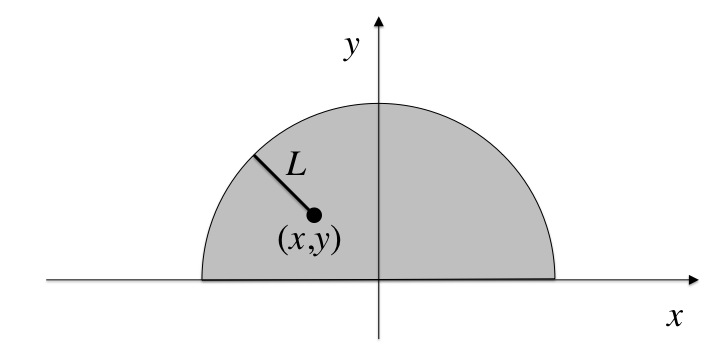
\includegraphics[width=0.65\textwidth]{ImgRadialCenterOfMass.jpg}
  \end{center}
 \begin{quote} \caption{\label{FigCircPlate}\small{The density of the plate at $(x,y)$ is equal to $L$.}}\end{quote}
\end{figure}
% ~~~~~~~~~~~~~~~~~~~~~~~~~~~~~~~~~~~~~~~~~~~~~~~~~~~~~~~~~~~~~~~~~~~~~~~~~~~~~~~~~
\item % CENTER OF MASS, CARDIOID
\Emph{Center of Mass of a 2D Plate, Cardioid} \\
Find the centroid of the plate of the region $D$ bounded by the centroid $r=a(1+\cos\theta)$, where $a$ is a constant. The region $D$ is shown in the figure below.  

When finding the centroid, you may use a symmetry argument to find $\bar{y}$ by inspection. To find $\bar{x}$, you may want to use the reduction formula
\begin{align*}
  \int \cos^n x \ dx = \frac{\sin x(\cos x)^{n-1}}{n}+\frac{n-1}{n} \int(\cos x)^{n-2} \ dx.
\end{align*}
\begin{figure}[H]
  \vspace{-1pt}
  \begin{center}
    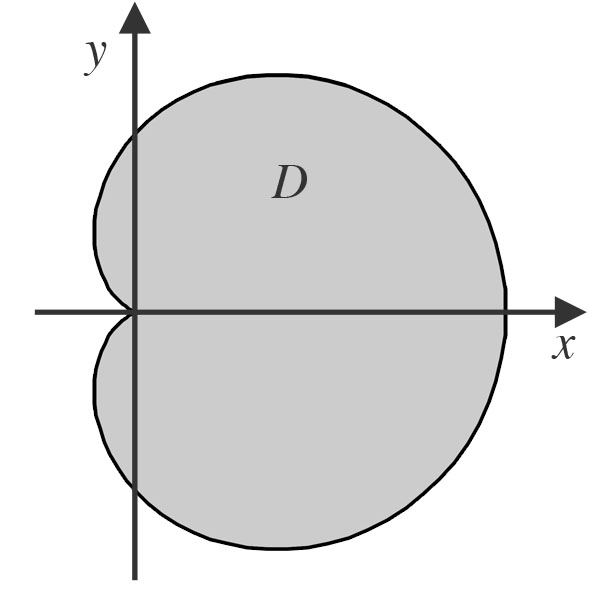
\includegraphics[width=0.35\textwidth]{ImgCardioid.jpg}
  \end{center}
 \begin{quote} \caption{\label{FigCircPlate}\small{The region $D$ is bounded by the cardioid $r=a(1+\cos\theta)$.}}\end{quote}
\end{figure}
% ~~~~~~~~~~~~~~~~~~~~~~~~~~~~~~~~~~~~~~~~~~~~~~~~~~~~~~~~~~~~~~~~~~~~~~~~~~~~~~~~~

\EEN % END OF SUBSECTION 





